\documentclass[journal]{IEEEtran}
\usepackage[spanish]{babel}
\usepackage[utf8]{inputenc}
\usepackage{enumerate}
\usepackage{graphicx}
\usepackage{booktabs}
\usepackage{physics}

\hyphenation{op-tical net-works semi-conduc-tor}


\begin{document}
\title{Movimiento Rectilineo Uniforme }

\author{Licenciatura en Física	\\
Universidad Nacional Autónoma de México - Facultad de Ciencias\\
Profesor: José Alfredo Morales Pérez\\
Ayud. Lab.	Miranda García Ávila\\
Integrantes: Jeshua Roberto Estrada Ocampo,~\IEEEmembership{424003085}\\
            
\thanks{}% <-this % stops a space
\thanks{}% <-this % stops a space
\thanks{}}

\markboth{Laboratorio de Mecánica}%
{Shell \MakeLowercase{\textit{et al.}}: Bare Demo of IEEEtran.cls for Journals}

\maketitle

\begin{abstract}
El presente reporte describe el experimento realizado para estudiar el movimiento rectilíneo uniforme (MRU) utilizando un riel de aire de baja fricción. Se llevaron a cabo mediciones de posición y tiempo de un carrito deslizándose a lo largo del riel para determinar la relación lineal entre estas variables. Los resultados obtenidos demuestran que el movimiento del carrito se ajusta a las predicciones teóricas del MRU, confirmando una velocidad constante a lo largo del recorrido. La precisión de los datos se ve mejorada gracias a la reducción significativa de la fricción en el sistema experimental. Este estudio proporciona una comprensión clara del MRU y sirve como base para futuros experimentos de cinemática.
\end{abstract}

\begin{IEEEkeywords}
Movimiento rectilíneo uniforme, Medición de tiempo y posición, Velocidad constante
\end{IEEEkeywords}

\IEEEpeerreviewmaketitle

\section{INTRODUCCIÓN}
\subsection{Planteamiento}

\IEEEPARstart  {E}l estudio del movimiento rectilíneo uniforme (MRU) es fundamental en la comprensión de la cinemática y las leyes que rigen el movimiento de los cuerpos. Este tipo de movimiento se caracteriza por una velocidad constante y una trayectoria rectilínea, lo que lo convierte en un punto de partida esencial para el análisis de movimientos más complejos. La práctica con un riel de aire de baja fricción permite reducir al mínimo los efectos de la fricción, proporcionando un entorno casi ideal para observar y medir el MRU. La justificación de esta práctica radica en la necesidad de validar experimentalmente las teorías cinemáticas mediante un sistema que minimiza las perturbaciones externas. Además, el uso de un riel de aire facilita la obtención de datos precisos y repetibles, esenciales para una comprensión profunda y detallada del MRU. Este experimento no solo refuerza conceptos teóricos, sino que también desarrolla habilidades prácticas en la manipulación de equipos y análisis de datos en el contexto de la física experimental.\\

\subsubsection{Objetivos Generales}

 - Simular las condiciones necesarias para poder generar un movimiento con velocidad constante
 y comprobar que se trata de movimiento rectilıneo uniforme (MRU)\\
 - Medir con ayuda de diferentes herramientas, que efectivamente se trata de un movimiento con velocidad constante, a través de comparar que en intervalos de tiempo iguales se miden velocidades iguales\\

\subsubsection{Objetivos particulares}
- Determinar la relación entre la posición y el tiempo para un objeto en MRU.
- Calcular la velocidad constante del carrito a lo largo del riel de aire.\\
- Evaluar la precisión de las mediciones obtenidas en el experimento.\\
- Comparar los resultados experimentales con las predicciones teóricas del MRU.\\


\subsubsection{Hipótesis}
Si un carrito se desliza sobre un riel de aire de baja fricción, entonces su movimiento seguirá las características del movimiento rectilíneo uniforme, es decir, mantendrá una velocidad constante a lo largo de su trayectoria. Esto se evidenciará mediante una relación lineal entre la posición y el tiempo, con una pendiente que representará la velocidad constante del carrito.

\section{MARCO TEÓRICO}
El estudio del movimiento rectilíneo uniforme (MRU) es uno de los primeros pasos en la comprensión de la cinemática, una rama de la física que describe el movimiento de los cuerpos sin considerar las fuerzas que lo producen. Para analizar el MRU, se asume que un objeto se desplaza a lo largo de una línea recta con una velocidad constante.\\
el movimiento rectilíneo uniforme se caracteriza por las siguientes propiedades:

Velocidad Constante: La magnitud de la velocidad no cambia con el tiempo.
Trayectoria Rectilínea: El movimiento ocurre a lo largo de una línea recta.

La posición x(t) de un objeto en movimiento rectilíneo uniforme en función del tiempo t se expresa como:

\begin{equation}\label{eq:1}
 x(t) = x_0 + vt
\end{equation}

x(t) es la posición del objeto en el tiempo de t, \(x_0\) es la posición inicial del objeto, v es la velocidad constante del objeto
y t es el tiempo transcurrido.
Esta ecuación se deriva del hecho de que la velocidad v es la tasa de cambio de laposición con respecto al tiempo

\begin{equation}\label{eq:3}
 v = \frac{dx}{dt}
\end{equation}

integrando esta ecuación con respecto al tiempo, se obtiene:

\begin{equation}\label{eq:4}
\int v \mathrm{d}x = \int \mathrm{d}x
\end{equation}

\begin{equation}\label{eq:4}
vt + x_0 = x
\end{equation}

conde c es la constante de integración, que corresponde a la posición inicial \(x_0\)

\begin{equation}\label{eq:4}
x = x_0 + vt
\end{equation}

Según los textos mencionados, los gráficos de posición vs. tiempo y de velocidad vs. tiempo son herramientas importantes para analizar el MRU:

En un gráfico de posición vs. tiempo (x-t), una línea recta con pendiente positiva indica un movimiento rectilíneo uniforme con velocidad constante.\\
En un gráfico de velocidad vs. tiempo (v-t), una línea horizontal indica que la velocidad es constante a lo largo del tiempo.




\section{ MATERIALES}
\begin{itemize}
\item riel de aire \item compresora de aire \item camara \item nivel de mano
\item Tripie \item Deslizador \item Cinta adhesiva
\item metro de madera
\item dos ligas
\item flexómetro

\end{itemize}

\section{DESARROLLO EXPERIMENTAL}
\begin{figure}[h]
    \centering
    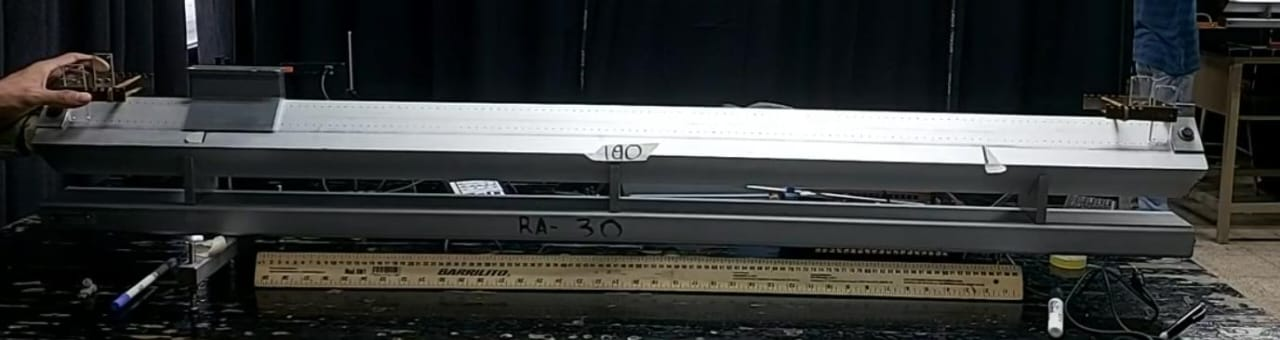
\includegraphics[width=1\linewidth]{Deslizador.png}
    \caption{Deslizador colocado horizontalmente}
    \label{fig:enter-label}
\end{figure}\\

Se amarra el hilo en el extremo superior de la base y en el otro extremo del hilo se amarra la peonza.\\
Una vez todo colocado, cómenzamos a realizar las mediciones, si utilizamos el cronómetro, tratar de ser lo más preciso, si se utiliza el sensor entonces asegurarse que la peonza esté a la altura en donde se pueda realizar el movimiento libremente y que el sensor sea capaz de detectarlo.\\
Para cambiar la longitud del péndulo, se enrrolla o se desenrolla el hilo. Para aumentae el peso de la peonza utilizamos plastilina colocandola en la parte superior de la peonza lo más uniforme posible.
\hfill 

\section{RESULTADOS}
\subsection{A continuación se presentan las gráficas obtenidas mediante el tracker.}

\begin{figure}[h]
    \centering
    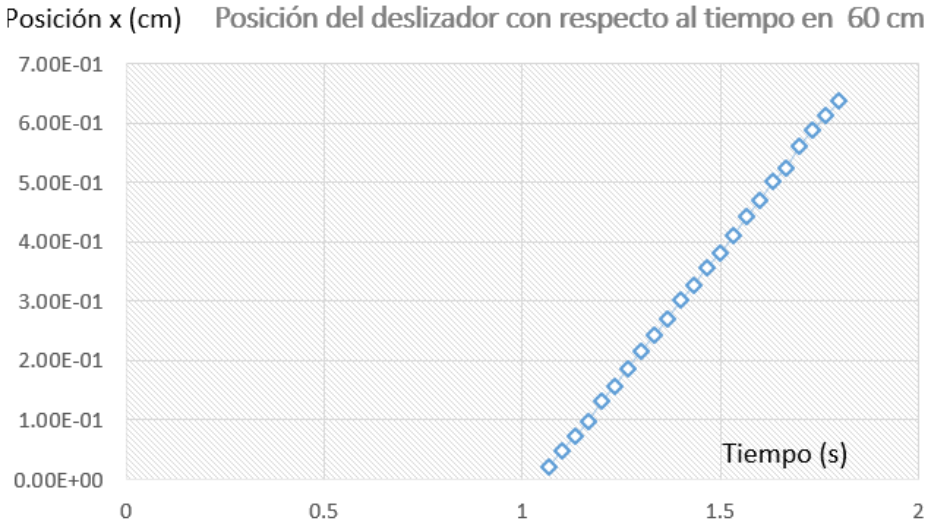
\includegraphics[width=1\linewidth]{graph1.png}
    \caption{Posición del deslizador con respecto al tiempo en 60 cm}
    \label{fig:enter-label}
\end{figure}\\

\begin{figure}[h]
    \centering
    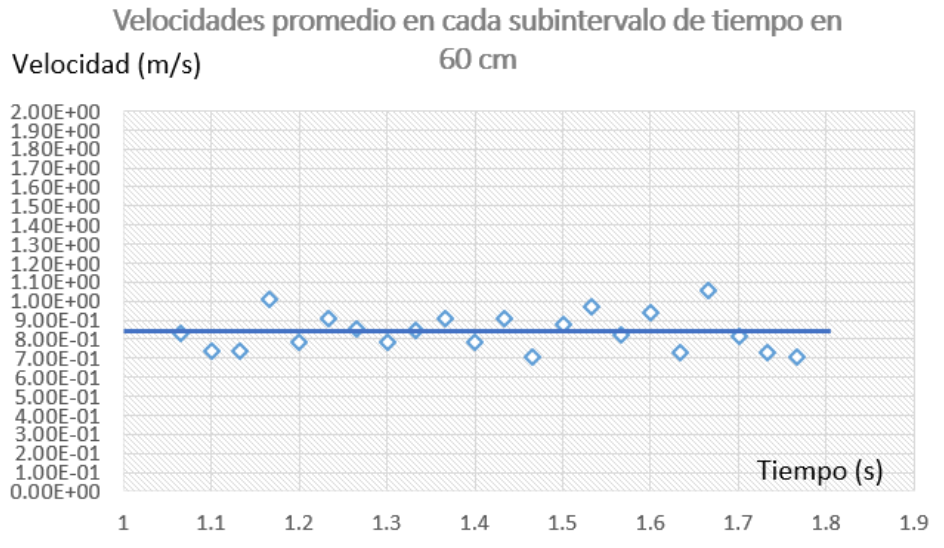
\includegraphics[width=1\linewidth]{graph2.png}
    \caption{Velocidades promedio en cada subintervalo de tiempo en 60 cm}
    \label{fig:enter-label}
\end{figure}\\

\newpage
\begin{figure}[h]
    \centering
    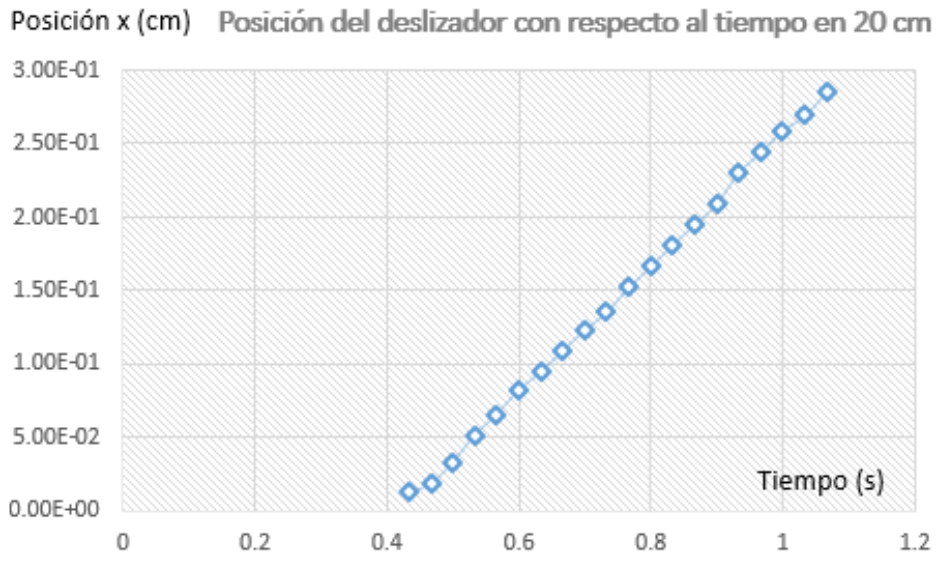
\includegraphics[width=1\linewidth]{graph3.png}
    \caption{Posición del deslizador con respecto al tiempo en 20 cm}
    \label{fig:enter-label}
\end{figure}\\

\newpage
\textit{}
\begin{figure}[h]
    \centering
    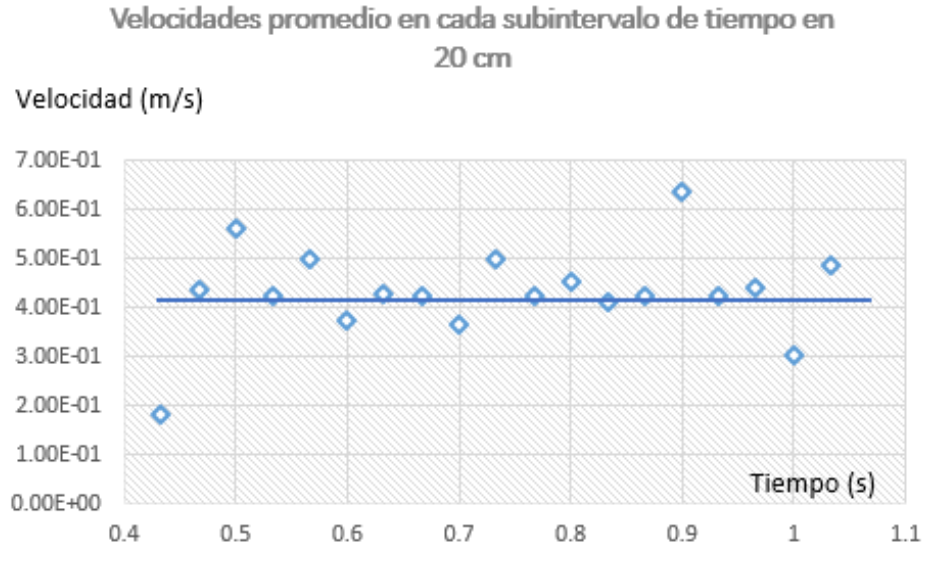
\includegraphics[width=1\linewidth]{graph4.png}
    \caption{Velocidades promedio en cada subintervalo de tiempo en 20 cm}
    \label{fig:enter-label}
\end{figure}\\\\
\textit{}\\
\begin{figure}[h]
    \centering
    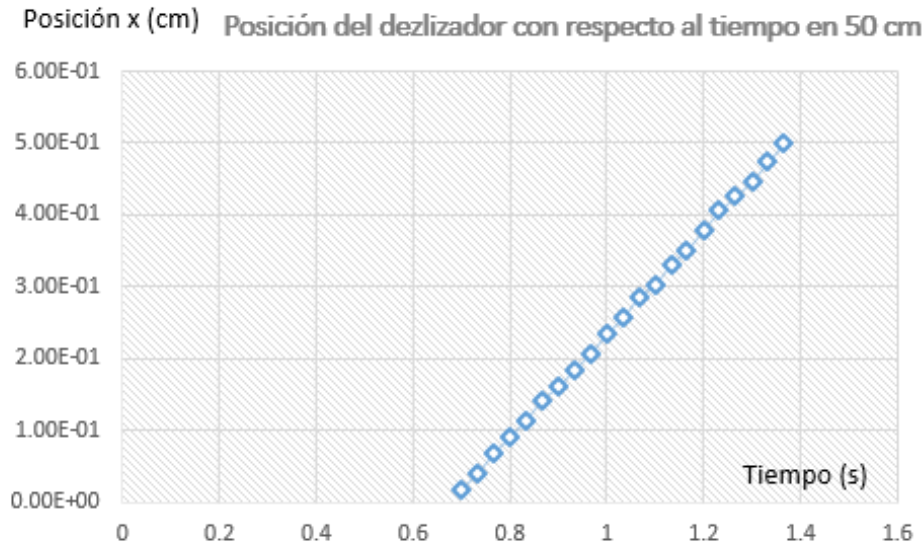
\includegraphics[width=1\linewidth]{graph5.png}
    \caption{Posición del deslizador con respecto al tiempo en 50 cm}
    \label{fig:enter-label}
\end{figure}\\\\
\textit{}\\
\begin{figure}[h]
    \centering
    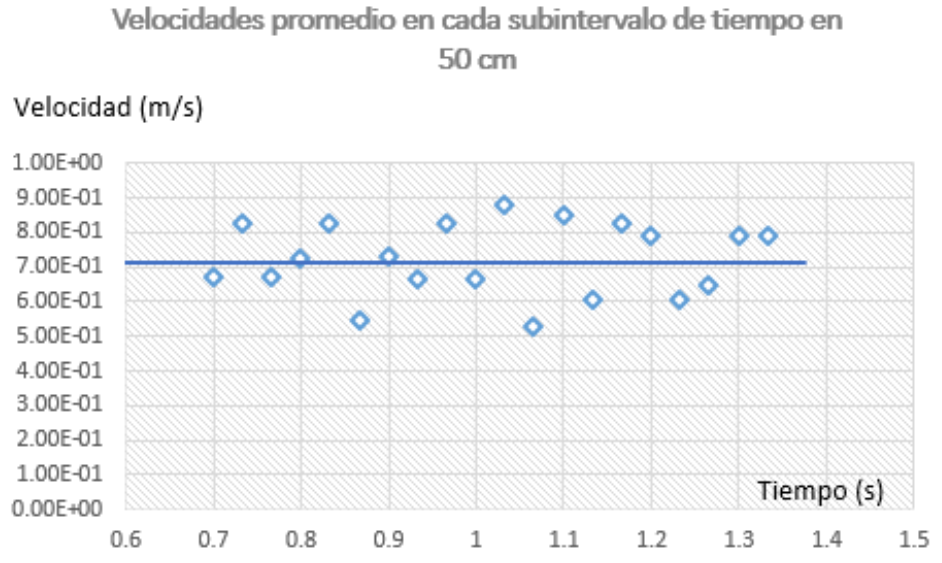
\includegraphics[width=1\linewidth]{graph6.png}
    \caption{Velocidades promedio en cada subintervalo de tiempo en 50 cm}
    \label{fig:enter-label}
\end{figure}\\

\begin{figure}[h]
    \centering
    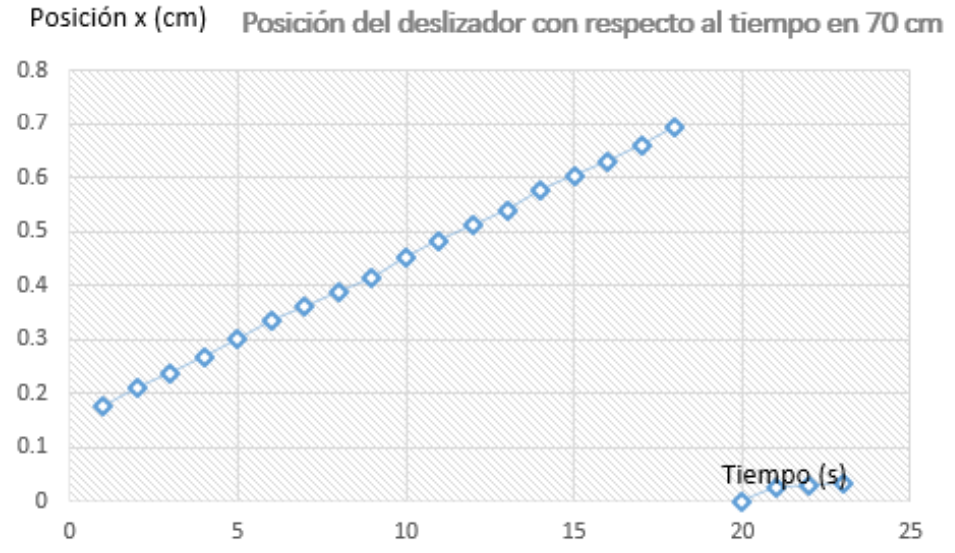
\includegraphics[width=1\linewidth]{graph7.png}
    \caption{Posición del deslizador con respecto al tiempo en 70 cm}
    \label{fig:enter-label}
\end{figure}\\\\
\textit{}\\
\newpage
\begin{figure}[h]
    \centering
    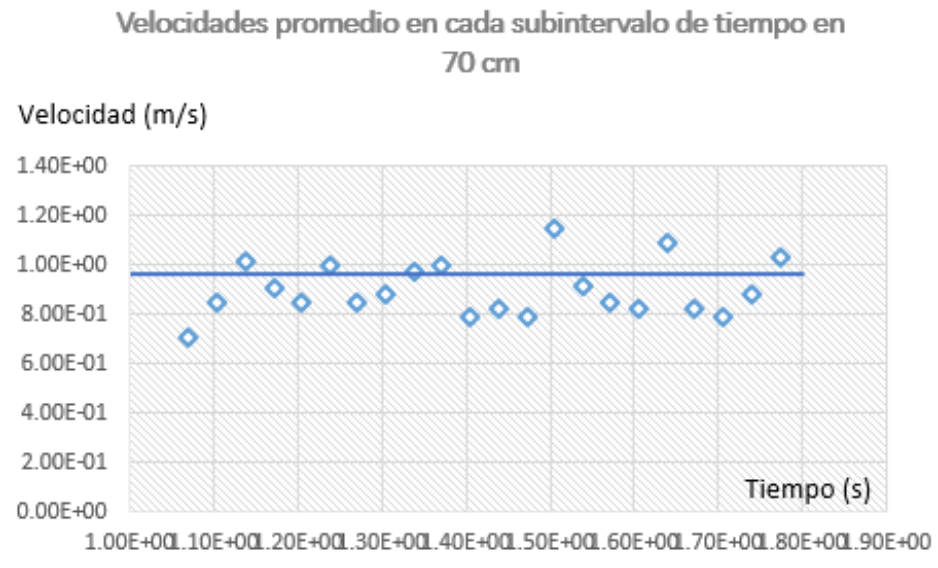
\includegraphics[width=1\linewidth]{graph8.png}
    \caption{Velocidades promedio en cada subintervalo de tiempo en 70 cm}
    \label{fig:enter-label}
\end{figure}\\\\
\textit{}\\
\begin{figure}[h]
    \centering
    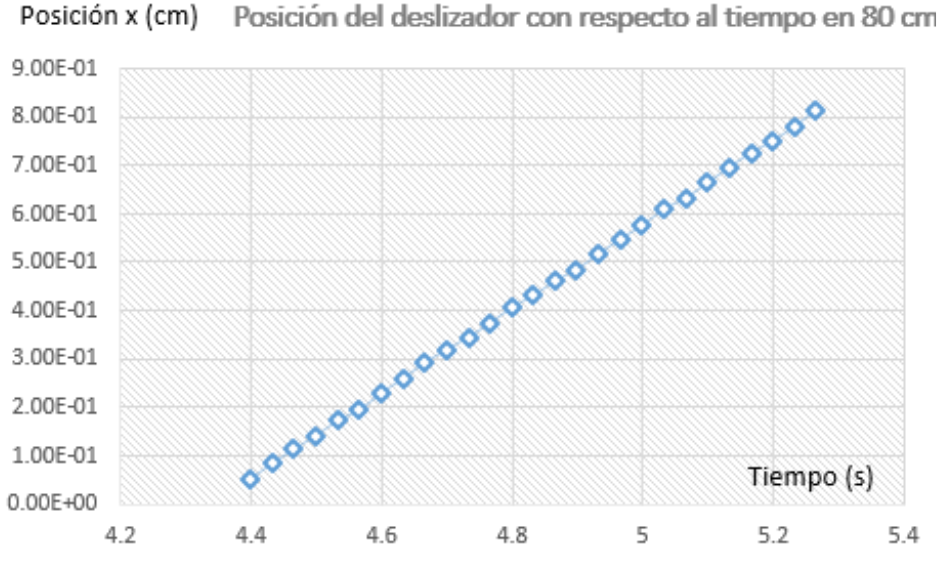
\includegraphics[width=1\linewidth]{graph9.png}
    \caption{Posición del deslizador con respecto al tiempo en 80 cm}
    \label{fig:enter-label}
\end{figure}\\
\newpage
\begin{figure}[h]
    \centering
    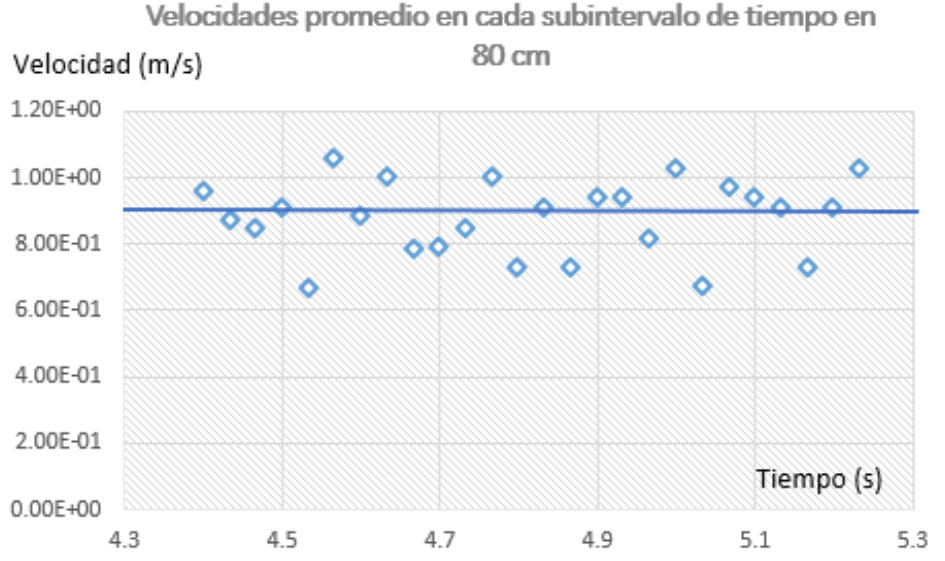
\includegraphics[width=1\linewidth]{graph10.png}
    \caption{Velocidades promedio en cada subintervalo de tiempo en 80 cm}
    \label{fig:enter-label}
\end{figure}\\

\begin{figure}[h]
    \centering
    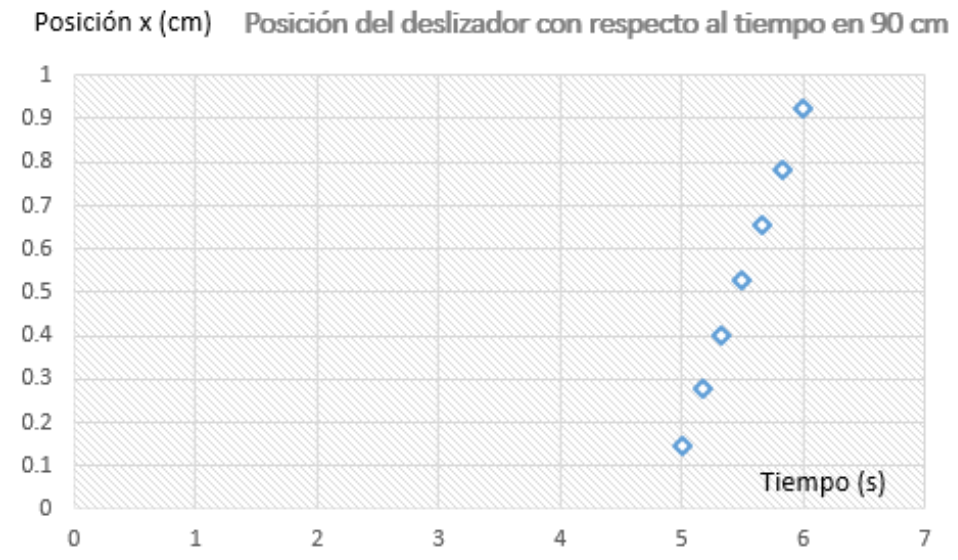
\includegraphics[width=1\linewidth]{graph11.png}
    \caption{Posición del deslizador con respecto al tiempo en 90 cm}
    \label{fig:enter-label}
\end{figure}

\begin{figure}[h]
    \centering
    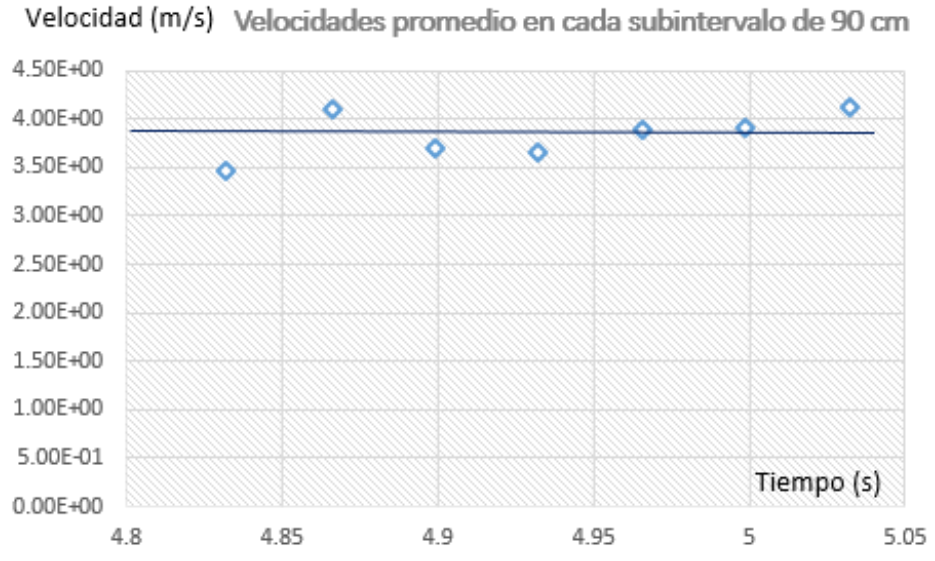
\includegraphics[width=1\linewidth]{graph12.png}
    \caption{Velocidades promedio en cada subintervalo de tiempo en 90 cm}
    \label{fig:enter-label}
\end{figure}\\\\
\newpage
\begin{figure}[h]
    \centering
    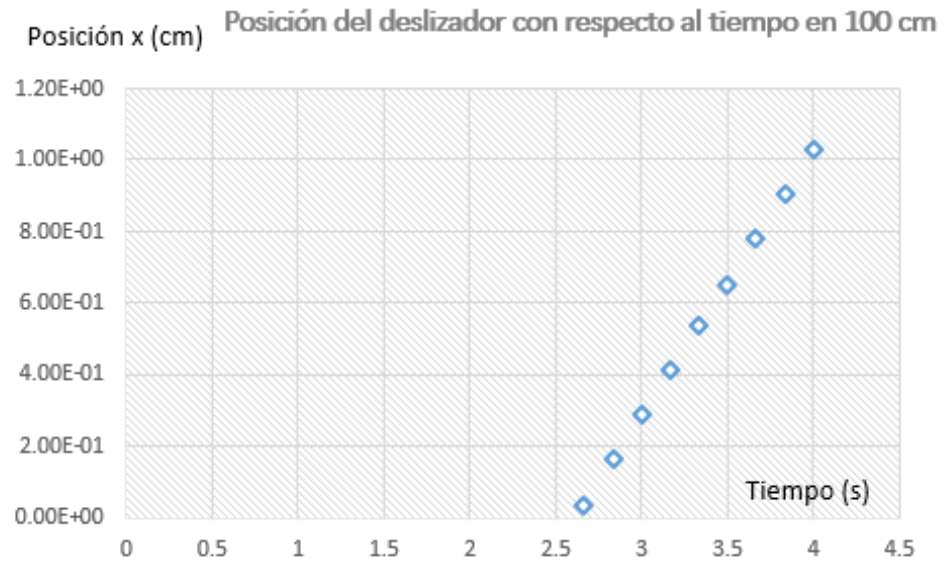
\includegraphics[width=1\linewidth]{graph13.png}
    \caption{Posición del deslizador con respecto al tiempo en 100 cm}
    \label{fig:enter-label}
\end{figure}\\

\begin{figure}[h]
    \centering
    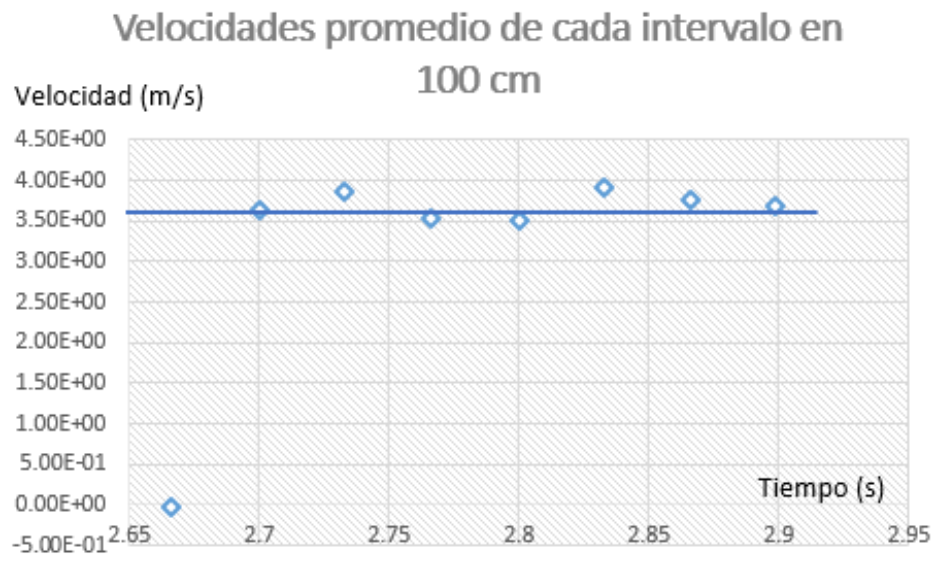
\includegraphics[width=1\linewidth]{graph14.png}
    \caption{Velocidades promedio en cada subintervalo de tiempo en 100 cm}
    \label{fig:enter-label}
\end{figure}\\

\section{DISCUSIÓN}
Considerando cada una de las tablas generadas a partir de las mediciones, se observa que para cada tiempo registrado por el software de análisis de video, la velocidad permanece aproximadamente constante (como se puede consultar en la sección de las tablas dedicada a las velocidades promedio, donde se muestra que el rango de desviación es muy pequeño) en cada intervalo de tiempo. Esto se aprecia visualmente en las versiones de velocidad de las gráficas presentadas después de las tablas de datos.\\\\

Es notable que, para las diferentes distancias seleccionadas, al calcular la velocidad promedio utilizando la ecuación (1) y los datos correspondientes a \(\Delta x\) y \(\Delta t\), el rango de variabilidad es muy pequeño para cada medida, sin importar la distancia en la que se realice la medición.\\\\

Las primeras gráficas (versiones de posición) demuestran, según nuestras hipótesis, que un movimiento rectilíneo uniforme requiere que la trayectoria descrita por el móvil sea una línea recta, lo cual se corrobora experimentalmente en estos gráficos.\\

Las versiones de velocidad de las diferentes mediciones equivalen a lo que obtendríamos si aplicáramos la ecuación (2), es decir, la derivada de la posición respecto al tiempo. Esto nos muestra que la tasa de cambio de la velocidad es nula, concordando con la hipótesis de que en un MRU la velocidad debe ser constante.\\\\

Es importante notar que los datos de las tablas y las gráficas marcadas con el símbolo (E) tienen un valor real de \(x \times 10^{-1}\), donde \(x\) es el valor proporcionado por el software de análisis de video. La incertidumbre se calculó contando el número de píxeles que abarcaba un centímetro de la regla en el video, dividiendo dos veces entre dos, ya que la escala mínima era de 0.5 cm, y su mitad se consideró como la incertidumbre en píxeles a reportar.


\section{ CONCLUSIONES} 
En consonancia con los objetivos inicialmente planteados:\\

Se logró simular de manera aproximada un movimiento con velocidad constante, comprobando que se trata de un movimiento rectilíneo uniforme (MRU). Esto se respaldó mediante el uso de la teoría pertinente, realizando los cálculos necesarios y analizando las gráficas obtenidas. \\

Se consiguió medir, con la ayuda de diversas herramientas, que efectivamente se trataba de un movimiento con velocidad constante. Esto se verificó al comparar intervalos de tiempo iguales, observando que las velocidades medidas eran constantes, además de tener en cuenta las incertidumbres e imperfecciones del experimento (errores sistemáticos y aleatorios). \\

Observaciones: Se sugiere que podrían haberse eliminado detalles como la variabilidad en los impulsos iniciales aplicados al deslizador, con el fin de simular siempre las mismas condiciones. Además, sería recomendable asegurar que la base del riel estuviera bien nivelada para minimizar las aceleraciones que podrían generarse debido a alguna inclinación.


% you can choose not to have a title for an appendix
% if you want by leaving the argument blank
\section{ REFERENCIAS}
\begin{itemize}
\item Serway, R. A., Jewett, J. W. (2008). "Física para ciencias e ingeniería.".
\item Resnick-Halliday. "Física Vol. 2, 5$^{ta}$ Edición, Editorial CECSA, México, 2005".
\item Aranzeta, C. G. (1986). "Introducción a la metodología experimental."
\item Oda-Noda, B. (2005). "Introducción al análisis gráfico de datos experimentales." 
\end{itemize}
% use section* for acknowledgment







\end{document}